\documentclass[a4paper,12pt]{article}

\usepackage[utf8x]{inputenc}
\usepackage[T2A]{fontenc}
\usepackage[english, russian]{babel}

% Опционно, требует  apt-get install scalable-cyrfonts.*
% и удаления одной строчки в cyrtimes.sty
% Сточку не удалять!
% \usepackage{cyrtimes}

% Картнки и tikz
\usepackage{graphicx}
\usepackage{tikz}
\usetikzlibrary{snakes,arrows,shapes}


% Некоторая русификация.
\usepackage{misccorr}
\usepackage{indentfirst}
\renewcommand{\labelitemi}{\normalfont\bfseries{--}}

% Увы, поля придётся уменьшить из-за листингов.
\topmargin -1cm
\oddsidemargin -0.5cm
\evensidemargin -0.5cm
\textwidth 17cm
\textheight 24cm

\sloppy

% Оглавление в PDF
\usepackage[
bookmarks=true,
colorlinks=true, linkcolor=black, anchorcolor=black, citecolor=black, menucolor=black,filecolor=black, urlcolor=black,
unicode=true
]{hyperref}

% Для исходного кода в тексте
\newcommand{\Code}[1]{\texttt{#1}}

\usepackage{verbatim}
\usepackage{fancyvrb}
\fvset{frame=leftline, fontsize=\small, framerule=0.4mm, rulecolor=\color{darkgray}, commandchars=\\\{\}}
\renewcommand{\theFancyVerbLine}{\small\arabic{FancyVerbLine}}


\title{Отчёт по лабораторной работе \\ <<Динамическая IP-маршрутизация>>}
\author{Федоров П.В.}

\begin{document}

\maketitle

\tableofcontents

\section{Настройка сети}

\subsection{Топология сети}

Топология сети и используемые IP-адреса показаны на рисунке~\ref{fig:network}.

\begin{figure}
\centering
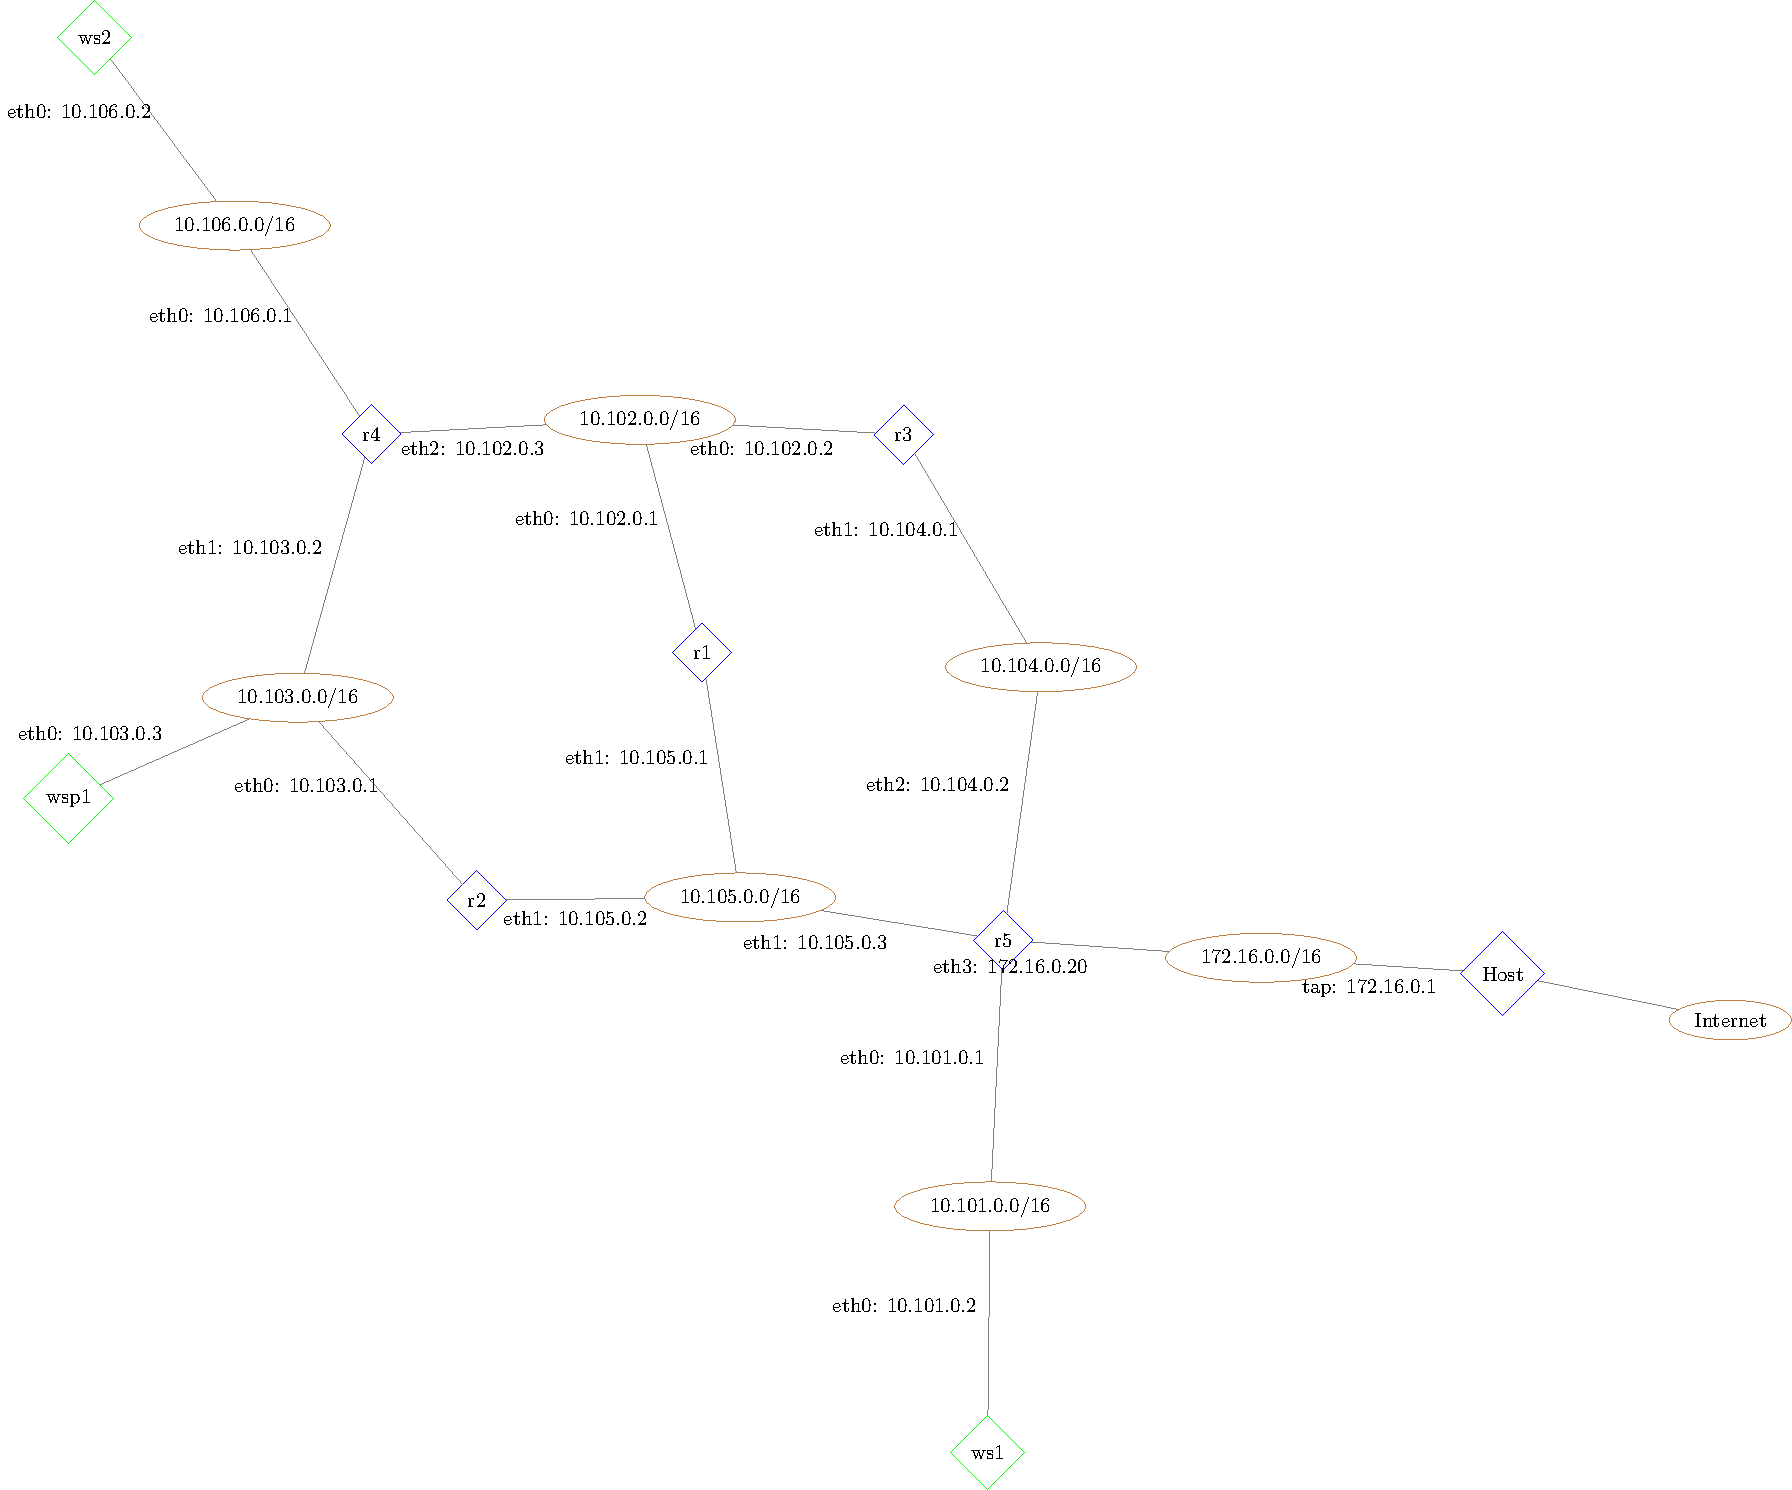
\includegraphics[width=0.8\textwidth]{includes/network_gv.pdf}
\caption{Топология сети}
\label{fig:network}
\end{figure}

Перечень узлов, на которых используется динамическая IP-маршрутизация:
\begin{enumerate}
    \item маршрутизатор \textbf{r1}
    \item маршрутизатор \textbf{r2}
    \item маршрутизатор \textbf{r3}
    \item маршрутизатор \textbf{r4}
    \item маршрутизатор \textbf{r5}
\end{enumerate}

\subsection{Назначение IP-адресов}

Сетевые настройки маршрутизатора \textbf{r1}.

\begin{Verbatim}
auto lo
iface lo inet loopback

auto eth0
iface eth0 inet static
address 10.102.0.1
netmask 255.255.0.0

auto eth1
iface eth1 inet static
address 10.105.0.1
netmask 255.255.0.0
\end{Verbatim}

Сетевые настройки маршрутизатора \textbf{r2}.

\begin{Verbatim}
auto lo
iface lo inet loopback

auto eth0
iface eth0 inet static
address 10.103.0.1
netmask 255.255.0.0

auto eth1
iface eth1 inet static
address 10.105.0.2
netmask 255.255.0.0
\end{Verbatim}

Сетевые настройки маршрутизатора \textbf{r3}.

\begin{Verbatim}
auto lo
iface lo inet loopback

auto eth0
iface eth0 inet static
address 10.102.0.2
netmask 255.255.0.0

auto eth1
iface eth1 inet static
address 10.104.0.1
netmask 255.255.0.0    
\end{Verbatim}

Сетевые настройки маршрутизатора \textbf{r4}.

\begin{Verbatim}
auto lo
iface lo inet loopback

auto eth0
iface eth0 inet static
address 10.106.0.1
netmask 255.255.0.0

auto eth1
iface eth1 inet static
address 10.103.0.2
netmask 255.255.0.0

auto eth2
iface eth2 inet static
address 10.102.0.3
netmask 255.255.0.0    
\end{Verbatim}

Сетевые настройки маршрутизатора \textbf{r5}.

\begin{Verbatim}
auto lo
iface lo inet loopback

auto eth0
iface eth0 inet static
address 10.101.0.1
netmask 255.255.0.0

auto eth1
iface eth1 inet static
address 10.105.0.3
netmask 255.255.0.0

auto eth2
iface eth2 inet static
address 10.104.0.2
netmask 255.255.0.0
\end{Verbatim}



Сетевые настройки рабочей станции \textbf{ws1}.

\begin{Verbatim}
auto lo
iface lo inet loopback

auto eth0
iface eth0 inet static
address 10.101.0.2
netmask 255.255.0.0
gateway 10.101.0.1    
\end{Verbatim}

Сетевые настройки рабочей станции \textbf{ws2}.

\begin{Verbatim}
auto lo
iface lo inet loopback

auto eth0
iface eth0 inet static
address 10.106.0.2
netmask 255.255.0.0
gateway 10.106.0.1
\end{Verbatim}

Сетевые настройки рабочей станции \textbf{wsp1}.

\begin{Verbatim}
auto lo
iface lo inet loopback

auto eth0
iface eth0 inet static
address 10.103.0.3
netmask 255.255.0.0
\end{Verbatim}

\subsection{Настройка протокола RIP}


Ниже приведен файл \Code{/etc/quagga/ripd.conf} маршрутизатора \textbf{r1}.

\begin{Verbatim}
router rip

network eth0
network eth1
    
timers basic 10 60 120
    
redistribute kernel
redistribute connected
    
log file /var/log/quagga/ripd.log    
\end{Verbatim}


Файл \Code{/etc/quagga/ripd.conf} маршрутизатора \textbf{r2}.

\begin{Verbatim}
router rip

network eth0
network eth1
    
timers basic 10 60 120
    
redistribute kernel
redistribute connected
    
log file /var/log/quagga/ripd.log    
\end{Verbatim}


Файл \Code{/etc/quagga/ripd.conf} маршрутизатора \textbf{r3}.

\begin{Verbatim}
router rip

network eth0
network eth1
    
timers basic 10 60 120
    
redistribute kernel
redistribute connected
    
log file /var/log/quagga/ripd.log    
\end{Verbatim}


Файл \Code{/etc/quagga/ripd.conf} маршрутизатора \textbf{r4}.

\begin{Verbatim}
router rip

network eth0
network eth1
network eth2

timers basic 10 60 120

redistribute kernel
redistribute connected

log file /var/log/quagga/ripd.log
\end{Verbatim}


Файл \Code{/etc/quagga/ripd.conf} маршрутизатора \textbf{r5} связанный с интернетом.

\begin{Verbatim}
router rip

network eth0
network eth1
network eth2

timers basic 10 60 120

redistribute kernel
! redistribute connected

log file /var/log/quagga/ripd.log
\end{Verbatim}


Ниже приведен файл \Code{/etc/quagga/ripd.conf} рабочий станции, связанной с несколькими маршрутизаторами \textbf{wsp1}.

\begin{Verbatim}
router rip

network eth0

timers basic 10 60 120

redistribute kernel
redistribute connected

log file /var/log/quagga/ripd.log    
\end{Verbatim}


\section{Проверка настройки протокола RIP}

Вывод \textbf{traceroute} от узла \textbf{ws1} до \textbf{ws2} при нормальной работе сети.

\begin{Verbatim}
traceroute -n 10.106.0.2 
traceroute to 10.106.0.2 (10.106.0.2), 64 hops max, 40 byte packets
    1  10.101.0.1  7 ms  0 ms  0 ms
    2  10.105.0.2  0 ms  0 ms  0 ms
    3  10.103.0.2  0 ms  0 ms  0 ms
    4  10.106.0.2  0 ms  1 ms  0 ms    
\end{Verbatim}

Вывод \textbf{traceroute} от узла \textbf{ws2} до \textbf{wsp1} при нормальной работе сети.

\begin{Verbatim}
traceroute -n 10.103.0.3
traceroute to 10.103.0.3 (10.103.0.3), 64 hops max, 40 byte packets
    1  10.106.0.1  0 ms  0 ms  0 ms
    2  10.103.0.3  2 ms  0 ms  0 ms    
\end{Verbatim}

Вывод \textbf{traceroute} от узла \textbf{ws2} до внешнего IP \textbf{10.0.2.2}.

\begin{Verbatim}
traceroute -n 10.0.2.2
traceroute to 10.0.2.2 (10.0.2.2), 64 hops max, 40 byte packets
	1  10.106.0.1  0 ms  3 ms  0 ms
	2  10.102.0.1  0 ms  0 ms  0 ms
	3  10.104.0.2  1 ms  0 ms  0 ms
	4  172.16.0.1  0 ms  0 ms  0 ms
	5  10.0.2.2  2 ms  2 ms  1 ms	
\end{Verbatim}
%падает основной сетевой интерфейс ноутбука
% 1: lo: <LOOPBACK,UP,LOWER_UP> mtu 65536 qdisc noqueue state UNKNOWN group default qlen 1000
%     link/loopback 00:00:00:00:00:00 brd 00:00:00:00:00:00
%     inet 127.0.0.1/8 scope host lo
%        valid_lft forever preferred_lft forever
%     inet6 ::1/128 scope host 
%        valid_lft forever preferred_lft forever
% 2: enp3s0: <NO-CARRIER,BROADCAST,MULTICAST,UP> mtu 1500 qdisc fq_codel state DOWN group default qlen 1000
%     link/ether 50:b7:c3:93:df:6a brd ff:ff:ff:ff:ff:ff
% 3: wlp2s0: <BROADCAST,MULTICAST,UP,LOWER_UP> mtu 1500 qdisc mq state UP group default qlen 1000
%     link/ether c8:f7:33:a3:38:fb brd ff:ff:ff:ff:ff:ff
%     inet 192.168.1.35/24 brd 192.168.1.255 scope global dynamic noprefixroute wlp2s0
%        valid_lft 25051sec preferred_lft 25051sec
%     inet6 fd6c:fe97:6714:0:bc62:86b9:ba2f:9120/64 scope global temporary dynamic 
%        valid_lft 604653sec preferred_lft 86010sec
%     inet6 fd6c:fe97:6714:0:218a:f829:6b29:eb0b/64 scope global dynamic mngtmpaddr noprefixroute 
%        valid_lft 4294319862sec preferred_lft 4294319862sec
%     inet6 fe80::5b14:9a3c:a079:fd1/64 scope link noprefixroute 
%        valid_lft forever preferred_lft forever
% 5: nk_tap_dafferru: <BROADCAST,MULTICAST,UP,LOWER_UP> mtu 1500 qdisc fq_codel state UP group default qlen 1000
%     link/ether b2:84:3d:6f:ee:23 brd ff:ff:ff:ff:ff:ff
%     inet 172.16.0.1/16 brd 172.16.255.255 scope global nk_tap_dafferru
%        valid_lft forever preferred_lft forever
%     inet6 fe80::b084:3dff:fe6f:ee23/64 scope link 
%        valid_lft forever preferred_lft forever

\subsection{Вывод сообщения RIP}

Вывод осуществлялся с помощью команды
\begin{Verbatim}
tcpdump -tnv -i ethNUM -s 1518 udp
\end{Verbatim}

Вывод сообщений RIP на маршрутизаторе \textbf{r2} с сетевого интерфейса \textbf{eth1}
\begin{verbatim}
    IP (tos 0x0, ttl 1, id 0, offset 0, flags [DF], proto UDP (17), length 72) 10.105.0.2.520 > 224.0.0.9.520:  
	RIPv2, Response, length: 44, routes: 2
	  AFI: IPv4:      10.103.0.0/16, tag 0x0000, metric: 1, next-hop: self
	  AFI: IPv4:      10.106.0.0/16, tag 0x0000, metric: 2, next-hop: self
IP (tos 0x0, ttl 1, id 0, offset 0, flags [DF], proto UDP (17), length 112) 10.105.0.3.520 > 224.0.0.9.520: 
	RIPv2, Response, length: 84, routes: 4
	  AFI: IPv4:         0.0.0.0/0 , tag 0x0000, metric: 1, next-hop: self
	  AFI: IPv4:      10.101.0.0/16, tag 0x0000, metric: 1, next-hop: self
	  AFI: IPv4:      10.102.0.0/16, tag 0x0000, metric: 2, next-hop: self
	  AFI: IPv4:      10.104.0.0/16, tag 0x0000, metric: 1, next-hop: self
IP (tos 0x0, ttl 1, id 0, offset 0, flags [DF], proto UDP (17), length 92) 10.105.0.1.520 > 224.0.0.9.520: 
	RIPv2, Response, length: 64, routes: 3
	  AFI: IPv4:      10.102.0.0/16, tag 0x0000, metric: 1, next-hop: self
	  AFI: IPv4:      10.104.0.0/16, tag 0x0000, metric: 2, next-hop: self
	  AFI: IPv4:      10.106.0.0/16, tag 0x0000, metric: 2, next-hop: self
IP (tos 0x0, ttl 1, id 0, offset 0, flags [DF], proto UDP (17), length 72) 10.105.0.2.520 > 224.0.0.9.520: 
	RIPv2, Response, length: 44, routes: 2
	  AFI: IPv4:      10.103.0.0/16, tag 0x0000, metric: 1, next-hop: self
	  AFI: IPv4:      10.106.0.0/16, tag 0x0000, metric: 2, next-hop: self
IP (tos 0x0, ttl 1, id 0, offset 0, flags [DF], proto UDP (17), length 112) 10.105.0.3.520 > 224.0.0.9.520: 
	RIPv2, Response, length: 84, routes: 4
	  AFI: IPv4:         0.0.0.0/0 , tag 0x0000, metric: 1, next-hop: self
	  AFI: IPv4:      10.101.0.0/16, tag 0x0000, metric: 1, next-hop: self
	  AFI: IPv4:      10.102.0.0/16, tag 0x0000, metric: 2, next-hop: self
	  AFI: IPv4:      10.104.0.0/16, tag 0x0000, metric: 1, next-hop: self
IP (tos 0x0, ttl 1, id 0, offset 0, flags [DF], proto UDP (17), length 92) 10.105.0.1.520 > 224.0.0.9.520: 
	RIPv2, Response, length: 64, routes: 3
	  AFI: IPv4:      10.102.0.0/16, tag 0x0000, metric: 1, next-hop: self
	  AFI: IPv4:      10.104.0.0/16, tag 0x0000, metric: 2, next-hop: self
	  AFI: IPv4:      10.106.0.0/16, tag 0x0000, metric: 2, next-hop: self
\end{verbatim}

Вывод таблицы RIP на \textbf{r2}.

\begin{Verbatim}
        Network         Next Hop         Metric From            Tag Time
R(n) 0.0.0.0/0          10.105.0.3            2 10.105.0.3        0 00:56
R(n) 10.101.0.0/16      10.105.0.3            2 10.105.0.3        0 00:56
R(n) 10.102.0.0/16      10.105.0.1            2 10.105.0.1        0 00:55
C(i) 10.103.0.0/16      0.0.0.0               1 self              0
R(n) 10.104.0.0/16      10.105.0.3            2 10.105.0.3        0 00:56
C(i) 10.105.0.0/16      0.0.0.0               1 self              0
R(n) 10.106.0.0/16      10.103.0.2            2 10.103.0.2        0 00:51    
\end{Verbatim}

Вывод таблицы маршрутизации.

\begin{Verbatim}
10.101.0.0/16 via 10.105.0.3 dev eth1  proto zebra  metric 2 
10.103.0.0/16 dev eth0  proto kernel  scope link  src 10.103.0.1 
10.102.0.0/16 via 10.105.0.1 dev eth1  proto zebra  metric 2 
10.105.0.0/16 dev eth1  proto kernel  scope link  src 10.105.0.2 
10.104.0.0/16 via 10.105.0.3 dev eth1  proto zebra  metric 2 
10.106.0.0/16 via 10.103.0.2 dev eth0  proto zebra  metric 2 
default via 10.105.0.3 dev eth1  proto zebra  metric 2     
\end{Verbatim}

\section{Расщепленный горизонт и испорченные обратные обновления}

Рассмотрим несколько выводов на одном маршрутизаторе с различной конфигурацией поддержки протокола \textbf{RIP}
В качестве маршрутизатора для эксперимента выступит маршрутизатор \textbf{r2}

\subsection{On: Split-horizon, Poisoned-reverse}
Для включения правил изменим \textbf{ripd.conf} на маршрутизаторе \textbf{r2}
\begin{verbatim}
interface eth0
ip rip split-horizon poisoned-reverse
\end{verbatim}

Вывод \textbf{tcpdump}

\begin{verbatim}
IP (tos 0x0, ttl 1, id 0, offset 0, flags [DF], proto UDP (17), length 132) 10.103.0.2.520 > 224.0.0.9.520: 
	RIPv2, Response, length: 104, routes: 5
	  AFI: IPv4:         0.0.0.0/0 , tag 0x0000, metric: 3, next-hop: self
	  AFI: IPv4:      10.101.0.0/16, tag 0x0000, metric: 3, next-hop: self
	  AFI: IPv4:      10.102.0.0/16, tag 0x0000, metric: 1, next-hop: self
	  AFI: IPv4:      10.104.0.0/16, tag 0x0000, metric: 2, next-hop: self
	  AFI: IPv4:      10.106.0.0/16, tag 0x0000, metric: 1, next-hop: self
IP (tos 0x0, ttl 1, id 0, offset 0, flags [DF], proto UDP (17), length 172) 10.103.0.1.520 > 224.0.0.9.520: 
	RIPv2, Response, length: 144, routes: 7
	  AFI: IPv4:         0.0.0.0/0 , tag 0x0000, metric: 2, next-hop: self
	  AFI: IPv4:      10.101.0.0/16, tag 0x0000, metric: 2, next-hop: self
	  AFI: IPv4:      10.102.0.0/16, tag 0x0000, metric: 16, next-hop: 10.103.0.2
	  AFI: IPv4:      10.103.0.0/16, tag 0x0000, metric: 16, next-hop: self
	  AFI: IPv4:      10.104.0.0/16, tag 0x0000, metric: 2, next-hop: self
	  AFI: IPv4:      10.105.0.0/16, tag 0x0000, metric: 1, next-hop: self
	  AFI: IPv4:      10.106.0.0/16, tag 0x0000, metric: 16, next-hop: 10.103.0.2
\end{verbatim}

Отметим, что маршрутизатор \textbf{r2} отправляет пакеты с указанием сетей полученных из данной сети (10.103.0.0/16) метрикой 16

\subsection{Off: split-horizon, poisoned-reverse}

Для включения правил изменим \textbf{ripd.conf} на маршрутизаторе \textbf{r2}
\begin{verbatim}
interface eth0
no ip rip split-horizon poisoned-reverse
\end{verbatim}

Вывод \textbf{tcpdump}

\begin{verbatim}
IP (tos 0x0, ttl 1, id 0, offset 0, flags [DF], proto UDP (17), length 112) 10.103.0.1.520 > 224.0.0.9.520: 
	RIPv2, Response, length: 84, routes: 4
	  AFI: IPv4:         0.0.0.0/0 , tag 0x0000, metric: 2, next-hop: self
	  AFI: IPv4:      10.101.0.0/16, tag 0x0000, metric: 2, next-hop: self
	  AFI: IPv4:      10.104.0.0/16, tag 0x0000, metric: 2, next-hop: self
	  AFI: IPv4:      10.105.0.0/16, tag 0x0000, metric: 1, next-hop: self
IP (tos 0x0, ttl 1, id 0, offset 0, flags [DF], proto UDP (17), length 132) 10.103.0.2.520 > 224.0.0.9.520: 
	RIPv2, Response, length: 104, routes: 5
	  AFI: IPv4:         0.0.0.0/0 , tag 0x0000, metric: 3, next-hop: self
	  AFI: IPv4:      10.101.0.0/16, tag 0x0000, metric: 3, next-hop: self
	  AFI: IPv4:      10.102.0.0/16, tag 0x0000, metric: 1, next-hop: self
	  AFI: IPv4:      10.104.0.0/16, tag 0x0000, metric: 2, next-hop: self
	  AFI: IPv4:      10.106.0.0/16, tag 0x0000, metric: 1, next-hop: self
\end{verbatim}

Отметим, что маршрутизатор \textbf{r2} отправляет пакеты с указанием сетей полученных из данной сети (10.103.0.0/16), но уже без указания пометки,
что данная сеть достижима с помощью маршрутизаторов сети, в которую происходит групповая передача данных

\section{Имитация устранимой поломки в сети}

В данном эксперименте будем задействовать 3 маршрутизатора
\begin{enumerate}
    \item маршрутизатор \textbf{r2} - отключаемый
    \item маршрутизатор \textbf{r3} - отключаемый
    \item маршрутизатор \textbf{r5} - для мониторинга устранимой поломки сети
\end{enumerate}

Проверим текущий путь от \textbf{ws1} до \textbf{ws2} не задействует маршрутизатор \textbf{r5} (пакет не проходит \textbf{10.105.0.0/16})
\begin{verbatim}
traceroute to 10.106.0.2 (10.106.0.2), 64 hops max, 40 byte packets
1  10.101.0.1  2 ms  0 ms  0 ms
2  10.104.0.1  11 ms  0 ms  0 ms
3  10.102.0.3  17 ms  1 ms  1 ms
4  10.106.0.2  17 ms  1 ms  1 ms   
\end{verbatim}

Для чистоты эксперимента и направлении трафика через единственный возможный путь выключим маршрутизаторы \textbf{r2} и \textbf{r3}
Таким образом останется единственный путь от \textbf{ws1} до \textbf{ws2} через \textbf{r5}

Перед отключением указанных маршрутизаторов рассмторим таблицу RIP на \textbf{r5}
\begin{verbatim}
K(r) 0.0.0.0/0          172.16.0.1            1 self              0
C(i) 10.101.0.0/16      0.0.0.0               1 self              0
R(n) 10.102.0.0/16      10.105.0.1            2 10.105.0.1        0 00:57
R(n) 10.103.0.0/16      10.105.0.2            2 10.105.0.2        0 00:52
C(i) 10.104.0.0/16      0.0.0.0               1 self              0
C(i) 10.105.0.0/16      0.0.0.0               1 self              0
R(n) 10.106.0.0/16      10.104.0.1            3 10.104.0.1        0 00:53    
\end{verbatim}

Отключим сетевые интерфейсы на маршрутизаторах \textbf{r2} \textbf{r3} (в случае отключения начинаются баги)

Мониторим таблицу

\textbf{Перед исчезновением}
\begin{verbatim}
     Network            Next Hop         Metric From            Tag Time
K(r) 0.0.0.0/0          172.16.0.1            1 self              0
C(i) 10.101.0.0/16      0.0.0.0               1 self              0
R(n) 10.102.0.0/16      10.105.0.1            2 10.105.0.1        0 00:51
R(n) 10.103.0.0/16      10.105.0.2            2 10.105.0.2        0 00:03
C(i) 10.104.0.0/16      0.0.0.0               1 self              0
C(i) 10.105.0.0/16      0.0.0.0               1 self              0
R(n) 10.106.0.0/16      10.104.0.1            3 10.104.0.1        0 00:00
\end{verbatim}

\textbf{Один из маршрутов invalid}
\begin{verbatim}
     Network            Next Hop         Metric From            Tag Time
K(r) 0.0.0.0/0          172.16.0.1            1 self              0
C(i) 10.101.0.0/16      0.0.0.0               1 self              0
R(n) 10.102.0.0/16      10.105.0.1            2 10.105.0.1        0 00:51
R(n) 10.103.0.0/16      10.105.0.2            2 10.105.0.2        0 00:03
C(i) 10.104.0.0/16      0.0.0.0               1 self              0
C(i) 10.105.0.0/16      0.0.0.0               1 self              0
R(n) 10.106.0.0/16      10.104.0.1           16 10.104.0.1        0 02:00
\end{verbatim}

\textbf{Найден новый путь}
\begin{verbatim}
     Network            Next Hop         Metric From            Tag Time
K(r) 0.0.0.0/0          172.16.0.1            1 self              0
C(i) 10.101.0.0/16      0.0.0.0               1 self              0
R(n) 10.102.0.0/16      10.105.0.1            2 10.105.0.1        0 00:58
R(n) 10.103.0.0/16      10.105.0.2           16 10.105.0.2        0 02:00
C(i) 10.104.0.0/16      0.0.0.0               1 self              0
C(i) 10.105.0.0/16      0.0.0.0               1 self              0
R(n) 10.106.0.0/16      10.105.0.1            3 10.105.0.1        0 00:58
\end{verbatim}
     
Вывод \textbf{traceroute} от узла \textbf{ws1} до \textbf{ws2} после того, как служба RIP перестроила таблицы маршрутизации.
\begin{Verbatim}
traceroute to 10.106.0.2 (10.106.0.2), 64 hops max, 40 byte packets
1  10.101.0.1  0 ms  0 ms  0 ms
2  10.105.0.1  0 ms  0 ms  0 ms
3  10.102.0.3  0 ms  0 ms  0 ms
4  10.106.0.2  0 ms  1 ms  1 ms
\end{Verbatim}

\section{Имитация неустранимой поломки в сети}

Для данного эксперимента будем прерывать соединения на маршрутизаторе \textbf{r4} тем самым сегмент сети с адресом \textbf{10.106.0.0/16}
станет недостижимым. 

Рассмотрим таблицу RIP на маршрутизаторе \textbf{r3} до отключения \textbf{r4}
\begin{verbatim}
     Network            Next Hop         Metric From            Tag Time
R(n) 0.0.0.0/0          10.104.0.2            2 10.104.0.2        0 00:53
R(n) 10.101.0.0/16      10.104.0.2            2 10.104.0.2        0 00:53
C(i) 10.102.0.0/16      0.0.0.0               1 self              0
R(n) 10.103.0.0/16      10.102.0.3            2 10.102.0.3        0 00:52
C(i) 10.104.0.0/16      0.0.0.0               1 self              0
R(n) 10.105.0.0/16      10.104.0.2            2 10.104.0.2        0 00:53
R(n) 10.106.0.0/16      10.102.0.3            2 10.102.0.3        0 00:52    
\end{verbatim}

запустим на \textbf{r1} tcpdump для отслеживания сообщений RIP протокола и отключим \textbf{r4}

После отключения наблюдаем следующую RIP таблицу на \textbf{r3}
\begin{verbatim}
     Network            Next Hop         Metric From            Tag Time
R(n) 0.0.0.0/0          10.104.0.2            2 10.104.0.2        0 00:52
R(n) 10.101.0.0/16      10.104.0.2            2 10.104.0.2        0 00:52
C(i) 10.102.0.0/16      0.0.0.0               1 self              0
R(n) 10.103.0.0/16      10.104.0.2            3 10.104.0.2        0 00:52
C(i) 10.104.0.0/16      0.0.0.0               1 self              0
R(n) 10.105.0.0/16      10.104.0.2            2 10.104.0.2        0 00:52
R(n) 10.106.0.0/16      10.102.0.3           16 10.102.0.3        0 01:47    
\end{verbatim}

Так же отметим что происходило на \textbf{r1}
\begin{verbatim}
IP (tos 0x0, ttl 1, id 0, offset 0, flags [DF], proto UDP (17), length 52) 10.102.0.3.520 > 224.0.0.9.520: 
	RIPv2, Response, length: 24, routes: 1
	  AFI: IPv4:      10.106.0.0/16, tag 0x0000, metric: 16, next-hop: self
IP (tos 0x0, ttl 1, id 0, offset 0, flags [DF], proto UDP (17), length 72) 10.102.0.3.520 > 224.0.0.9.520: 
	RIPv2, Response, length: 44, routes: 2
	  AFI: IPv4:      10.103.0.0/16, tag 0x0000, metric: 1, next-hop: self
	  AFI: IPv4:      10.106.0.0/16, tag 0x0000, metric: 16, next-hop: self
IP (tos 0x0, ttl 1, id 0, offset 0, flags [DF], proto UDP (17), length 52) 10.102.0.3.520 > 224.0.0.9.520: 
	RIPv2, Response, length: 24, routes: 1
	  AFI: IPv4:      10.103.0.0/16, tag 0x0000, metric: 16, next-hop: self
\end{verbatim}
Отметим что сеть \textbf{10.106.0.0/16} недостижима о чем свидетельствует метрика 16 в 1 RIP ответе

Ниже приведена таблица RIP на \textbf{r1}
\begin{verbatim}
     Network            Next Hop         Metric From            Tag Time
R(n) 0.0.0.0/0          10.105.0.3            2 10.105.0.3        0 00:57
R(n) 10.101.0.0/16      10.105.0.3            2 10.105.0.3        0 00:57
C(i) 10.102.0.0/16      0.0.0.0               1 self              0
R(n) 10.103.0.0/16      10.105.0.2            2 10.105.0.2        0 00:51
R(n) 10.104.0.0/16      10.105.0.3            2 10.105.0.3        0 00:57
C(i) 10.105.0.0/16      0.0.0.0               1 self              0
\end{verbatim}

И таблица маршрутизации
\begin{verbatim}
10.101.0.0/16 via 10.105.0.3 dev eth1  proto zebra  metric 2 
10.103.0.0/16 via 10.105.0.2 dev eth1  proto zebra  metric 2 
10.102.0.0/16 dev eth0  proto kernel  scope link  src 10.102.0.1 
10.105.0.0/16 dev eth1  proto kernel  scope link  src 10.105.0.1 
10.104.0.0/16 via 10.105.0.3 dev eth1  proto zebra  metric 2 
default via 10.105.0.3 dev eth1  proto zebra  metric 2 
\end{verbatim}

\end{document}